\documentclass[tikz,border=0.1cm]{standalone}
\usepackage{tikz}
\usetikzlibrary{bayesnet}
\usepackage{amsmath,amsthm}
\usepackage{amssymb}
\usepackage{amsfonts}
\tikzset{>=latex}

\begin{document}
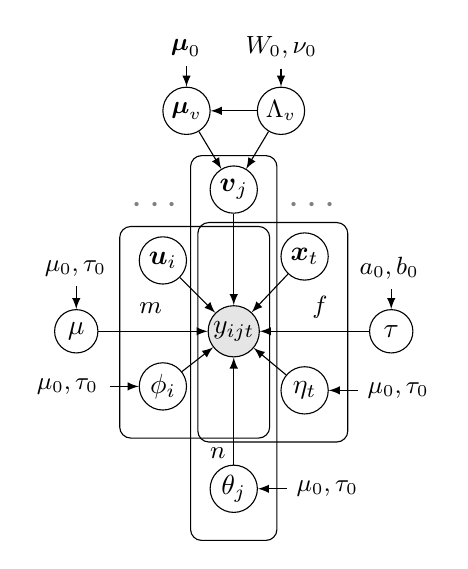
\begin{tikzpicture}
\node[circle,draw=black,fill=gray!20,inner sep=0pt,minimum size=0.65cm] (obs) at (2,-1) {{$y_{ijt}$}};
\node[circle,draw=black,inner sep=0pt,minimum size=0.6cm] (ui) at (1.1,-0.1) {{$\boldsymbol{u}_{i}$}};
\node[circle,draw=black,inner sep=0pt,minimum size=0.6cm] (vj) at (2,0.8) {{$\boldsymbol{v}_{j}$}};
\node[circle,draw=black,inner sep=0pt,minimum size=0.6cm] (xt) at (2.9,-0.05) {{$\boldsymbol{x}_{t}$}};
\node[circle,draw=black,inner sep=0pt,minimum size=0.6cm] (phi) at (1.1,-1.7) {{$\phi_{i}$}};
\node[circle,draw=black,inner sep=0pt,minimum size=0.6cm] (theta) at (2,-3) {{$\theta_{j}$}};
\node[circle,draw=black,inner sep=0pt,minimum size=0.6cm] (eta) at (2.9,-1.75) {{$\eta_{t}$}};
\node[circle,draw=black,inner sep=0pt,minimum size=0.55cm] (tau) at (4.0,-1) {{$\tau$}};
\node[circle,draw=black,inner sep=0pt,minimum size=0.55cm] (mu) at (0,-1) {{$\mu$}};
\path [draw,->] (ui) edge (obs);
\path [draw,->] (vj) edge (obs);
\path [draw,->] (xt) edge (obs);
\path [draw,->] (tau) edge (obs);
\path [draw,->] (mu) edge (obs);
\path [draw,->] (phi) edge (obs);
\path [draw,->] (theta) edge (obs);
\path [draw,->] (eta) edge (obs);
\node [text width=0.2cm] (m) at (0.9,-0.7) {\small{$m$}};
\plate[] {plate1} {(obs)(ui)(m)(phi)} { };
\node [text width=0.6cm] (n) at (2,-2.55) {\small{$n$}};
\plate[] {plate2} {(obs)(vj)(n)(theta)} { };
\node [text width=0.2cm] (f) at (3.1,-0.7) {\small{$f$}};
\plate[] {plate3} {(obs)(xt)(f)(eta)} { };
\node[circle,draw=black,inner sep=0pt,minimum size=0.6cm] (muv) at (1.4,1.8) {\small{$\boldsymbol{\mu}_{v}$}};
\node[circle,draw=black,inner sep=0pt,minimum size=0.6cm] (lambdav) at (2.6,1.8) {\small{$\Lambda_{v}$}};
\node[text width=0.8cm] (gamma) at (4.0,-0.2) {\small{$a_0,b_0$}};
\node[text width=0.8cm] (hyper1) at (0,-0.2) {\small{$\mu_{0},\tau_{0}$}};
\node[text width=0.8cm] (hyper2) at (3.2,-3) {\small{$\mu_{0},\tau_{0}$}};
\node[text width=0.8cm] (hyper3) at (4.1,-1.75) {\small{$\mu_{0},\tau_{0}$}};
\node[text width=0.8cm] (hyper4) at (-0.1,-1.7) {\small{$\mu_{0},\tau_{0}$}};
\node[text width=0.4cm] (mu0) at (1.4,2.6) {\small{$\boldsymbol{\mu}_{0}$}};
\node[text width=0.9cm] (wnu0) at (2.6,2.6) {\small{$W_{0},\nu_{0}$}};
\node[text width=0.6cm] (cdots1) at (1,0.6) {\Large\color{gray}{$\cdots$}};
\node[text width=0.6cm] (cdots2) at (3,0.6) {\Large\color{gray}{$\cdots$}};
\path [draw,->] (muv) edge (vj);
\path [draw,->] (lambdav) edge (vj);
\path [draw,->] (lambdav) edge (muv);
\path [draw,->] (mu0) edge (muv);
\path [draw,->] (wnu0) edge (lambdav);
\path [draw,->] (gamma) edge (tau);
\path [draw,->] (hyper1) edge (mu);
\path [draw,->] (hyper2) edge (theta);
\path [draw,->] (hyper3) edge (eta);
\path [draw,->] (hyper4) edge (phi);
\end{tikzpicture}
\end{document}
